\chapter{Methodology}
\label{sec:latexumg}

\section{Global description of the algorithm}
\label{sec:gliederung}

The Algorithm can be divided into four main steps : 
\begin{enumerate}
    \item Preprocessing : segments the vegetation from its background
    \item Hough Transform : extracts the main lines of the image  
    \item Outlier line detection : using the vanishing point, eliminates the lines that are not crossing at that point and replaces them with the next most prominent lines in the image
    \item RANSAC : using points around mask corresponding to the regions around the lines previously detected, calculates the center of the crops
\end{enumerate}

The complete algorithm can be visualized in Fig. \ref{pics:AlgoFlowChart}. \\

The algorithm works on single images or sequences of images. As the Hough transform is computationally expensive, the algorithm doesn't use it at each frame : at the end of the RANSAC process, the region of the crops for the next frame is updated : as low changed between each frame was considered, the region where the crops were on the previous frame is used as a reference. As long as the crops detected are considered "valid", only the RANSAC process is runned again, the vanishing point staying the same. 

Frames are considered invalid if two crops are too close to each other, if two crops have too similar an angle, if a crop has an angle too close to the horizon, if there are too few vegetation pixels in the area of the crops detected in the previous frame, or if the frame number is a multiple of K (K can be adapted according to the precision needed).

\begin{figure}
   \centering
   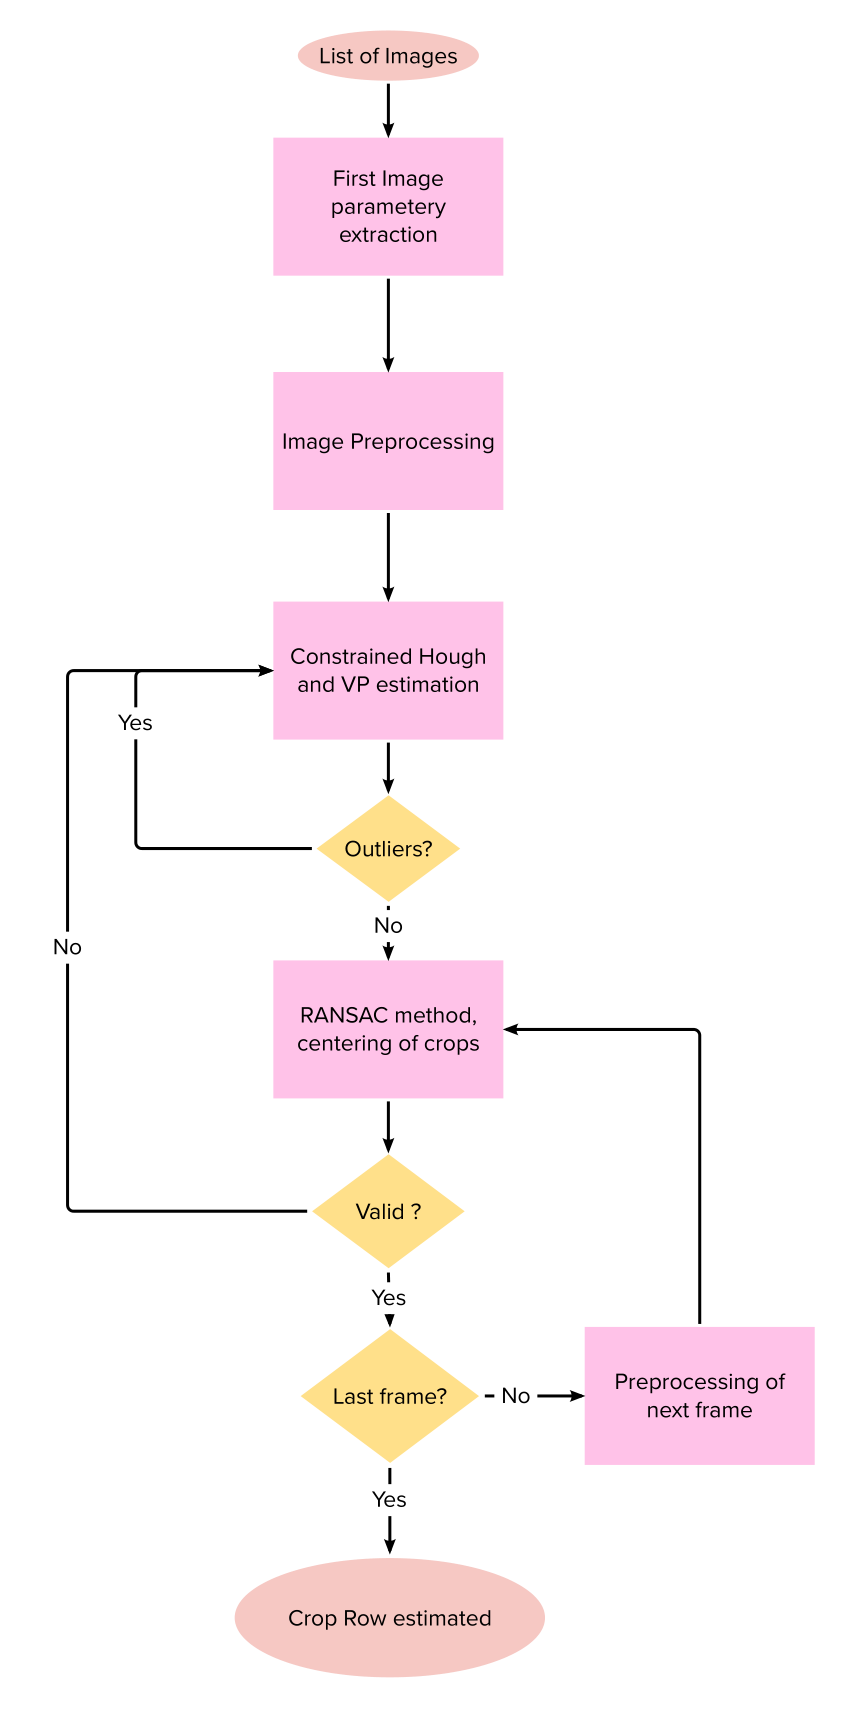
\includegraphics[width=0.75\textwidth]{Report/images/FlowCharts/Algo14_01_2023-01-16_13-58-50.png}
   \caption{Flowchart of the Algorithm}
   \label{pics:AlgoFlowChart}
\end{figure}

\section{Image Preprocessing : sky extraction and vegetation segmentation}
\label{sec:gliederung}

The Preprocessing part of the algorithm serves many purposes:
\begin{enumerate}
    \item Extracts and resizes images
    \item Removes the sky
    \item Removes the extremely bushy regions
    \item Clusters the main colours and extracts the greenest one
    \item Masks the image using a custom threshold on this colour 
    \item Depending on the density of the segmented vegetation, calculates edges of the image or keeps the entire image before proceeding with the first Hough Transform
    \end{enumerate}

\subsubsection{Sky Removal}

This step reduces the Region of Interest of our image to speed up the algorithm. Results are shown in Fig. \ref{eq:my_equation} It consists of three main parts: 

\begin{itemize} 
  \item Laplacian Calculation and thresholding : the Laplacian (the second derivative of the image) is calculated to identify edges and fine details. Pixels with low Laplacian are kept -these are the areas of small changes, which should represent the sky.
  \item Horizon Line Detection : after median filter is applied per column, the first pixels of each column with a high level of change are memorized.
  \item Elimination of non-sky regions : Starting from the top row, the algorithm eliminates horizontal rows until it finds a row where a line is composed of less than 50\% sky (low Laplacian pixels).
\end{itemize}

\begin{figure}[H]
\centering
\begin{subfigure}{0.49\textwidth}
    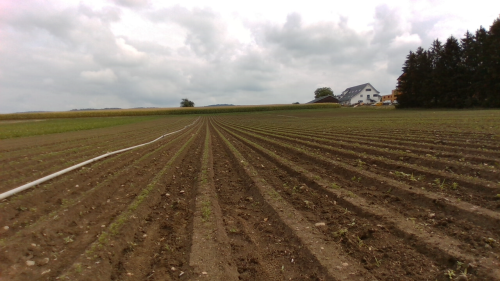
\includegraphics[width=\textwidth]{Report/images/IMGWITHSKY.png}
    \label{fig:first}
\end{subfigure}
\begin{subfigure}{0.49\textwidth}%
    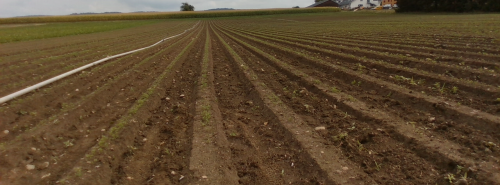
\includegraphics[width=\textwidth]{Report/images/IMGNOSKY.png}
    \label{fig:second}
\end{subfigure}
\caption{Results of the sky removal algorithm}
\end{figure}
\label{pics: Vegewithandwithoutsky}

\subsubsection{Colour Clustering, vegetation colour extraction}

As the vegetation’s colour varies a lot depending on the lighting, a threshold for the vegetation index isn't robust enough. 

K clusters of colors are created by counting the number of pixels with the same color in an image. The color with the highest pixel count is grouped with all other colors that have a difference in LAB space less than a certain threshold. This process is repeated for the second highest pixel count color, and so on, until K clusters are formed. The outcome can be seen in figure \ref{pics:ColourClus}.

\begin{figure}[H]
   \centering
   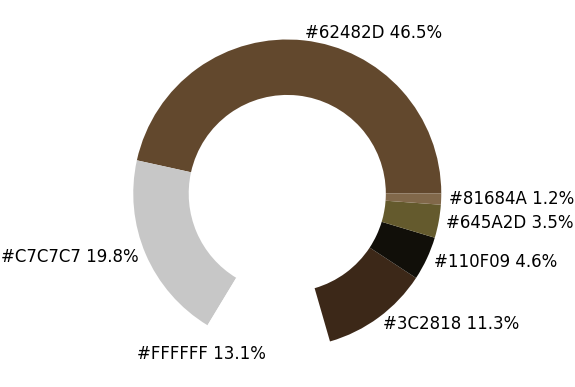
\includegraphics[width=0.75\textwidth]{images/donut.png}
   \caption{Visualisation of the clustered colour}
   \label{pics:ColourClus}
\end{figure}

The algorithm compares the clustered colors to the color with the norm closest  to [0, 255, 0] (lime in RGB space) in LAB space. This color is used to create a mask for the image and segment the vegetation by retaining all pixels with a LAB space difference under a certain threshold. \\

%TODO : maybe do tab at the end with all the hyperparameters values ?

In the video mode of the algorithm, the assumption is made that the color of the vegetation does not change much throughout the video. The reference vegetation color is calculated in frame 0. Although the reference color does not change, the threshold used during masking does, as the goal is to maintain the same level of information throughout the video (the ratio of 1-pixels to 0-pixels in the binary image being used to define "information."). The threshold value is adapted based on this ratio: if the ratio is smaller than the one in frame 0, the threshold is increased, and vice versa. This allows the algorithm to quickly segment the vegetation while maintaining the same level of information throughout the process. Recalculating the reference color at each frame is possible, but this technique has shown satisfactory results, is less computationally expensive, and is more stable. 

\begin{figure}[H]
\centering
\begin{subfigure}{0.49\textwidth}
    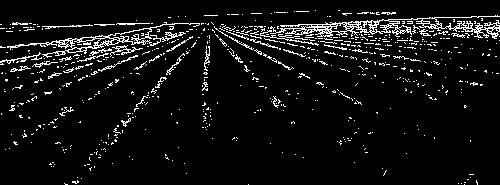
\includegraphics[width=\textwidth]{Report/images/VEGEIMG5.png}
    \label{fig:first}
\end{subfigure}
\begin{subfigure}{0.49\textwidth}%
    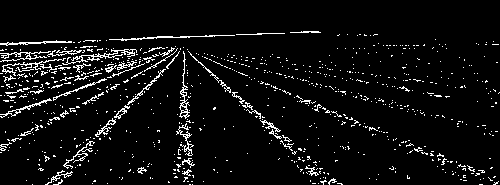
\includegraphics[width=\textwidth]{Report/images/VEGEIMG500.png}
    \label{fig:second}
\end{subfigure}
\caption{Vegetation Image of frame 5 and frame 500}
\end{figure}
\label{pics: Vegestablealongtime}

\subsubsection{Bushy Region Removal}

The image is eroded by a kernel proportional to its size. This new image is then subtracted from the original image. Results can be shown in Fig. \ref{pics: bushyremoval} 

\begin{figure}[H]
\centering
\begin{subfigure}{0.49\textwidth}
    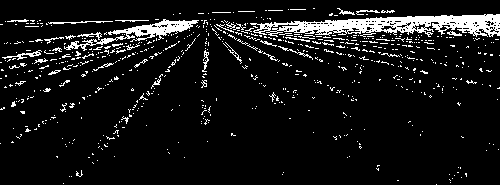
\includegraphics[width=\textwidth]{Report/images/IMGALLBUSHES.png}
    \label{fig:first}
\end{subfigure}
\begin{subfigure}{0.49\textwidth}%
    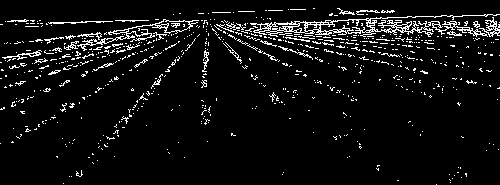
\includegraphics[width=\textwidth]{Report/images/IMGNOBUSHES.png}
    \label{fig:second}
\end{subfigure}
\caption{Erosion of the bushy regions}
\end{figure}
\label{pics: bushyremoval}

\section{First approximation of the crop rows : Hough Transform}
\label{sec:gliederung}

Our interest in the Hough Transform is two-fold : the lines are both used to calculate the vanishing point and to isolate the regions where the crop rows should be found in the RANSAC part of the algorithm. \\

\begin{figure}[h!]
\begin{minipage}{0.48\columnwidth}
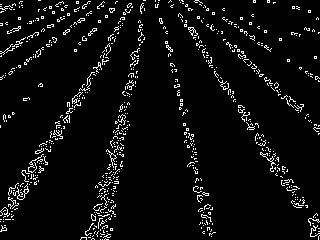
\includegraphics[width=\columnwidth,height=4cm]{Report/images/beforelineremoval.png.png}
\\[3mm]
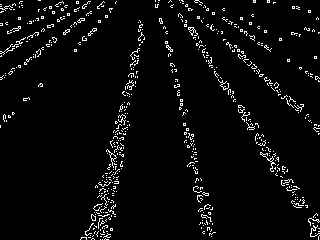
\includegraphics[width=\columnwidth,height=4cm]{Report/images/afterlineremoval.png}
\end{minipage}
\hspace{0.15\columnwidth}
\begin{minipage}{0.3\columnwidth}
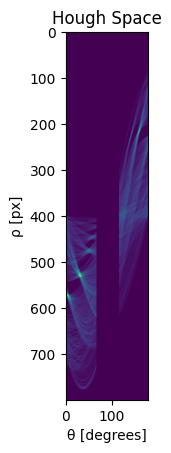
\includegraphics[width=\columnwidth,height=83mm]{Report/images/ImageProcesses/HoughSpacePerso/HTwithlabelconstraint.png}

\end{minipage}
\caption{Illustration of the Hough process}
\label{pics:diffHT}

\end{figure}


The Hough Transform described in \ref{subsubsection:HT} finds all the lines in the image with values in the accumulator greater than a certain threshold.

To ensure that the lines detected are spaced by a minimum threshold and no angle is the same, the algorithm implemented in this project uses a slightly different Hough transform.\\

Depending on the density of the vegetation, either the entire binary image or the edges of the binary image are taken (if the vegetation pixels are more then 10\% of the entire pixels) to accelerate the process.

Instead of using a threshold to take all lines, the N-maximums of the Hough space are extracted, where N is the number of desired rows. N is set to a defined number but the algorithm  can decrease this number if not enough lines satisfying the "crop conditions" are detected (as further explained in section \ref{sec:VPdet}). This approach allows the algorithm to be independent of a threshold.

When in Hough space, the maximum values to be selected must satisfy the following conditions : 
\begin{enumerate}
    \item No crops should have the same angle : this is done by putting a 0-band in the Hough space around each previously detected angle (cf Fig \ref{pics:diffHT}).
    \item Each 1-pixels should be used only once, to detect a line of a single row. This is done by masking the surroundings of where a line has been detected (cf Fig. \ref{pics:diffHT}). 
\end{enumerate}

Deletion of lines and angles is done iteratively.\\

This process ensures no crops are detected twice, but doesn't prevent detecting lines that are not going towards the vanishing point. 




\section{Vanishing Point Calculation and outliers elimination}
\label{sec:VPdet}

\begin{figure}[H]
   \centering
   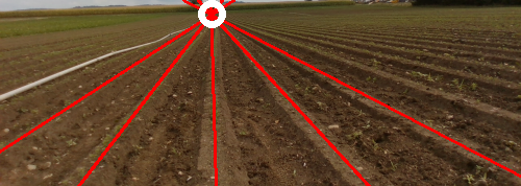
\includegraphics[width=0.75\textwidth]{Report/images/VPdetected.png}
   \caption{Vanishing Point detected}
   \label{pics:VPillu}
\end{figure}

This step makes sure that the lines in camera coordinates detected using the Hough transform all go towards the vanishing point, representing parallel lines in the world coordinates.\\

It is worth noting that the calculation of the vanishing point could in the future be used for other tasks, such as camera calibration, depth estimation, and perspective distortion correction. \\ 

\begin{figure}[H]
   \centering
   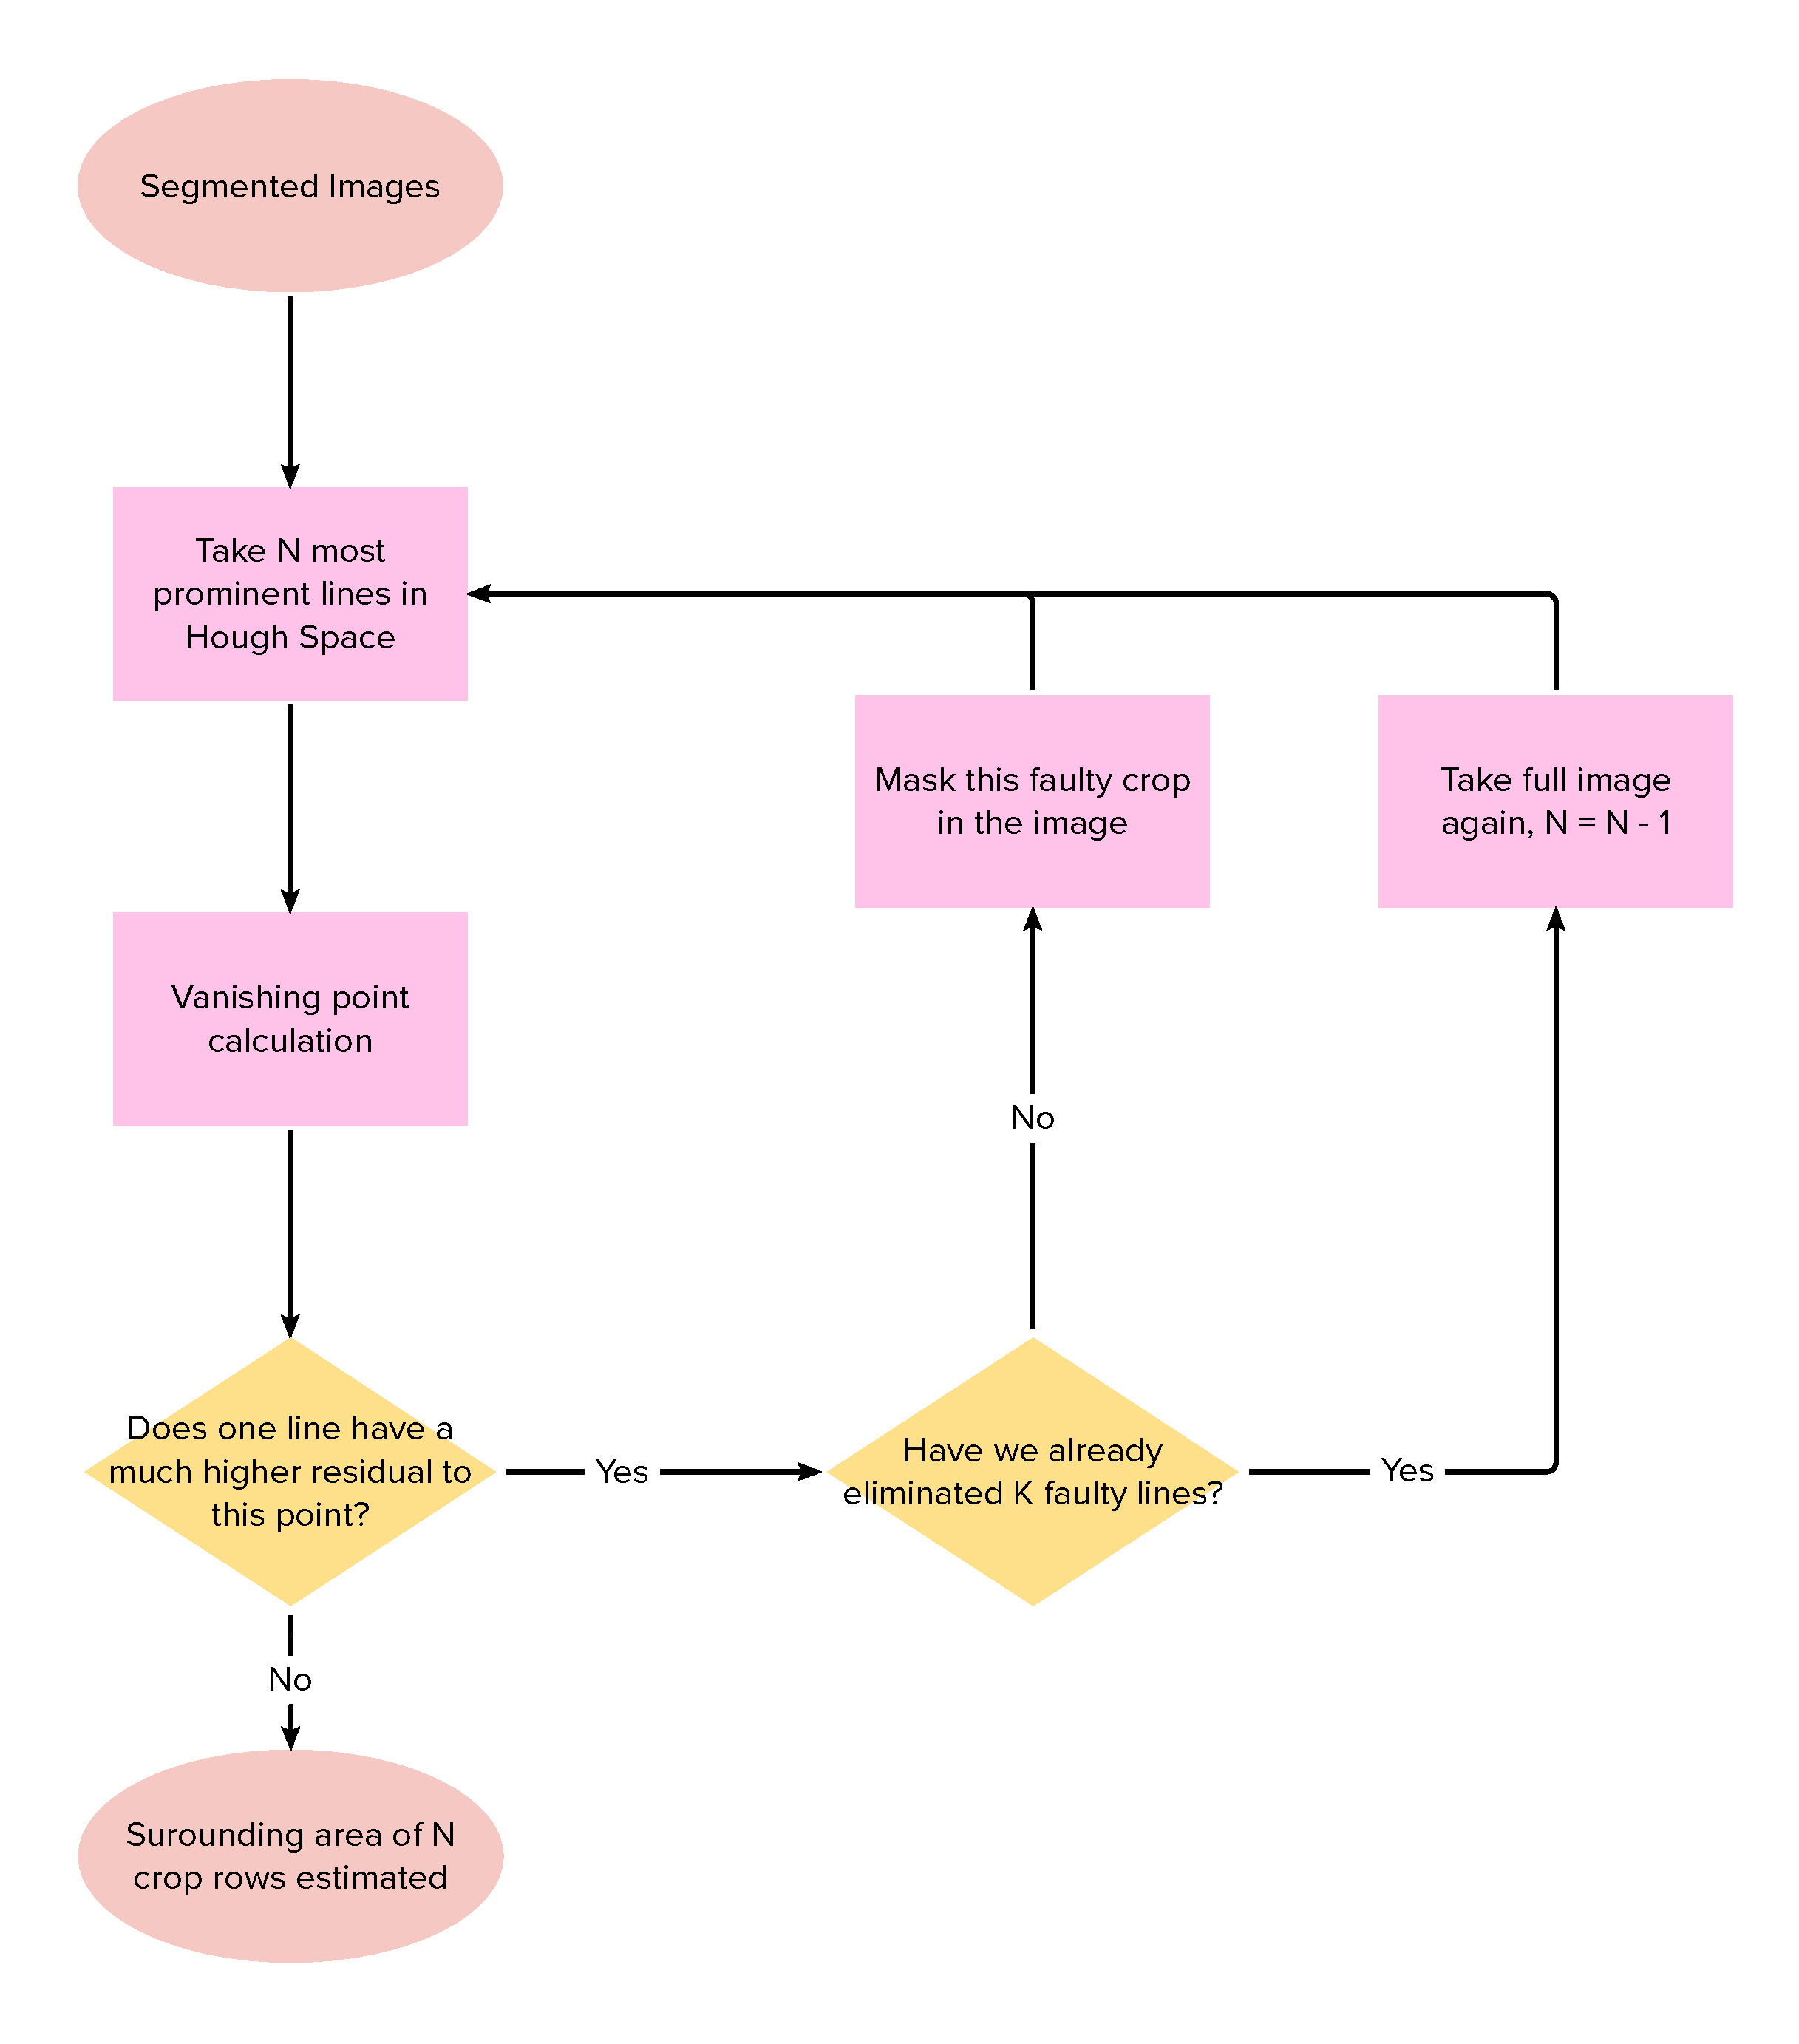
\includegraphics[width=0.75\textwidth]{Report/images/FlowCharts/VP calculation algorithm_2023-01-16_13-54-35.pdf}
   \caption{Flowchart of the Hough Process and Vanishing Point Calculation}
   \label{pics:VPCALC}
\end{figure}

Here, as it was proposed in \cite{CPCalcinHS}, the vanishing point is determined in the Hough Space and a iterative process is set up to eliminate outlier lines.  \\

As mentioned before, a point in the plane image is represented by a sinusoidal in the Hough space, which corresponds to all possible lines that could pass through this point. Thus, all the parallel lines in the world which pass through the vanishing point in the image plane should be on the same sinusoidal in the Hough space. Finding this sinusoidal should therefore describe the vanishing point in the following way:

\begin{equation}
\rho(\theta) = x_{0} \cdot \cos{\theta} + y_{0} \cdot \sin{\theta} = P(x_{0}, y_{0},\Phi) \cdot \sin{\theta + \Phi(x_{0}, y_{0})} .
 	\label{eq:my_equation}
\end{equation}

with : 
\begin{equation}
\begin{cases} 
P = x_{0}\cos(\Phi) \cdot \sin(1 + y_{0}^2/x_{0}^2) \\
\Phi = \arctan{y_{0}/x_{0}}
\end{cases}
 	\label{eq:my_equation}
\end{equation} \\

In the developed algorithm, a deterministic method is obviously not enough, as all parallel lines in the real world do not cross exactly at a single point, and as there could be "outlier" lines, not corresponding to parallel crops in the real world. The following statistical method was thus used :  


\begin{enumerate}
  \item Extract the dominant sinusoidal in the Hough space to get a first estimate of the vanishing point. This is done by solving the following minimisation problem : 
  
  \begin{equation}
\min_{x_{0}, y_{0}} \sum_{i=1}^{n} W_{i}(\rho_{i} - x_{0} \cos(\theta_{i}) - y_{0} \sin(\theta_{i}))^2
 	\label{eq:my_equation}
\end{equation}

Solving it leads to: 


\begin{equation}
  D_{it} =
    \begin{cases}
    A x_0 + C y_0 = D \\
    C x_0 + B y_0 = E
    \end{cases}       
\end{equation}

with : 
\begin{equation}
    \begin{cases}
      A = \sum_{i=1}^{n} W_{i} \cdot \cos{\theta_{i}}^2 \\
      B = \sum_{i=1}^{n} W_{i}\cdot  \sin{\theta_{i}}^2 \\
      C = \sum_{i=1}^{n} W_{i} \cdot \sin{\theta_{i}} \cdot \cos{\theta_{i}} \\
      D = \sum_{i=1}^{n} W_{i} \cdot \rho_i \cdot \cos{\theta_{i}}     \\
      E = \sum_{i=1}^{n} W_{i} \cdot \rho_i \cdot \sin{\theta_{i}}   \\

      \end{cases}
\end{equation}

  \item Once this point is found, compute the total variance of all lines with respect to this point : 
\begin{equation}
    \sigma^2 = \sum_{i=1}^{n} W_{i}  \epsilon_i^2
\end{equation}
    with : %TODO : rho en gras!!
\begin{equation}
    \epsilon_i =  \boldsymbol{\rho} -  \overline{\rho_{i}} 
\end{equation}

  
  \item If one of the lines is much more distant than this variance, that is \(\epsilon>k* \sigma\), classify it as an outlier and remove it from the detected line lists. An example of such a line is shown in Fig. \ref{pics:outlier}
  \item If more than k lines have already been detected as outliers, start detecting N-1 lines.
  \item Repeat the process: take the next dominant line in Hough space if N is unchanged, use the new set of lines to recalculate the vanishing point, and eliminate more outliers if necessary. 
  \item Stop when no more outliers are detected.

\end{enumerate}

A more concise explanation of this part can be visualized in Fig. \ref{pics:VPCALC}


\begin{figure}[H]
   \centering
   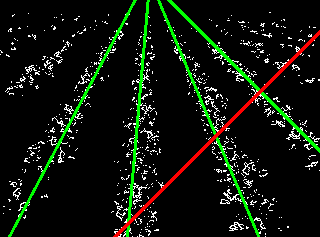
\includegraphics[width=0.65\textwidth]{Report/images/outlierdetected.png}
   \caption{Outlier line detected, soon to be eliminated}
   \label{pics:outlier}
\end{figure}





\section{Final detection : constrained RANSAC}
\label{sec:gliederung}

Once the estimate of the crop row position is estimated with the Hough transform and the vanishing point is calculated, RANSAC is used to fit lines in the center of the crop rows. Each fitted line uses a masked version of the vegetation segmented image, where only the regions surrounding the previously detected lines are kept, as shown in Fig. \ref{pics: Ransacmasking}. \\

\begin{figure}[H]
\centering
\begin{subfigure}{0.3\textwidth}
    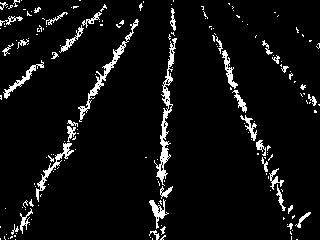
\includegraphics[width=\textwidth]{Report/images/VEGSEG.png}
    \caption{Vegetation image}
    \label{fig:first}

\end{subfigure}
\begin{subfigure}{0.3\textwidth}%
    
\includegraphics[width=\textwidth]{Report/images/CROPMASK.png}
    \caption{Mask used}
    \label{fig:second}

\end{subfigure}
\begin{subfigure}{0.3\textwidth}%
    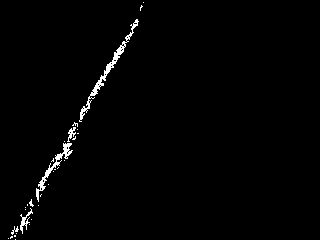
\includegraphics[width=\textwidth]{Report/images/VEGCROPSEG.png}
    \caption{Segmented crop row}
    \label{fig:third}

\end{subfigure}

\caption{Segmentation of a single crop row}
\end{figure}
\label{pics: Ransacmasking}



In this project, two approaches were tried to fit the rows with RANSAC : 


\begin{itemize}
  \item Fit the crops between the surrounding region of the vanishing point previously calculated and the surroundings of the lines detected with the Hough transform. As a personalized Python version of the RANSAC function was used, the process took a lot of time. It also needed additional iterations to find the best model, as an extra parameter was needed (the vanishing point's surroundings).
  
  \item Fit a single crop around the surrounding region of a line detected with the Hough transform, with a heavy bias towards the vanishing point - for this, the data points used for fitting a single line are augmented with multiple times the vanishing point coordinates - this method was selected for the final process, as it was faster and gave similar results.
\end{itemize}

There are two benefits to using RANSAC instead of the Hough transform :
\begin{enumerate}
  \item Hough transform is too slow for real-time application, using RANSAC on most frames and Hough only when necessary speeds up the crop row detection process. 
  \item The lines fitted with the Hough Algorithm are not necessarily the centers of the crops : when working with the edges of the image, they will even be fitted to the side of the crops. The data used for RANSAC being selected randomly from all the points of the crops, the lines detected are likely to be the center of the crops. 
\end{enumerate} 


\begin{figure}[H]
\centering
\begin{subfigure}{0.49\textwidth}
    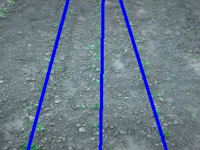
\includegraphics[width=\textwidth]{Report/images/houghdetection.png}
    \caption{Hough detection process, lines not fitted in the center }
    \label{fig:first}
\end{subfigure}
\begin{subfigure}{0.49\textwidth}%
    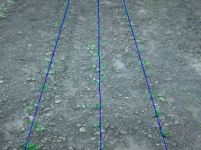
\includegraphics[width=\textwidth]{Report/images/ransacdetection.png}
    \caption{Ransac detection process, lines centered on the crops}
    \label{fig:second}
\end{subfigure}

\caption{Comparaison Hough and Ransac Process}
\end{figure}
\label{pics: HoughVSRansac}





 







